\documentclass[]{article}
\usepackage[margin=0.25in]{geometry}
\usepackage{pgfplots}
\pgfplotsset{width=10cm,compat=1.9}

\usepgfplotslibrary{external}
\tikzexternalize

\begin{document}
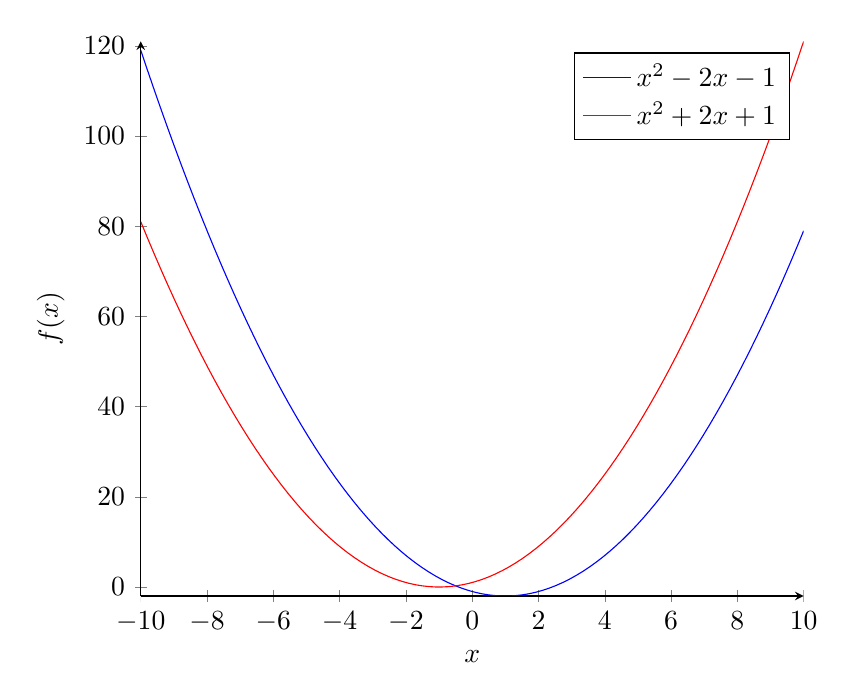
\begin{tikzpicture}
\begin{axis}[axis lines=left,xlabel=\(x\),ylabel={\(f(x)\)},]%set the axis only on the left and bottom sides of the plot, instead of the default box. 
\addplot[domain=-10:10,samples=100,color=blue,]{x^2-2*x-1};
\addlegendentry{\(x^2 - 2x - 1\)}
\addplot[domain=-10:10,samples=100,color=red,]{x^2+2*x+1};
\addlegendentry{\(x^2 + 2x + 1\)}
\end{axis}
\end{tikzpicture}

%plotting from data
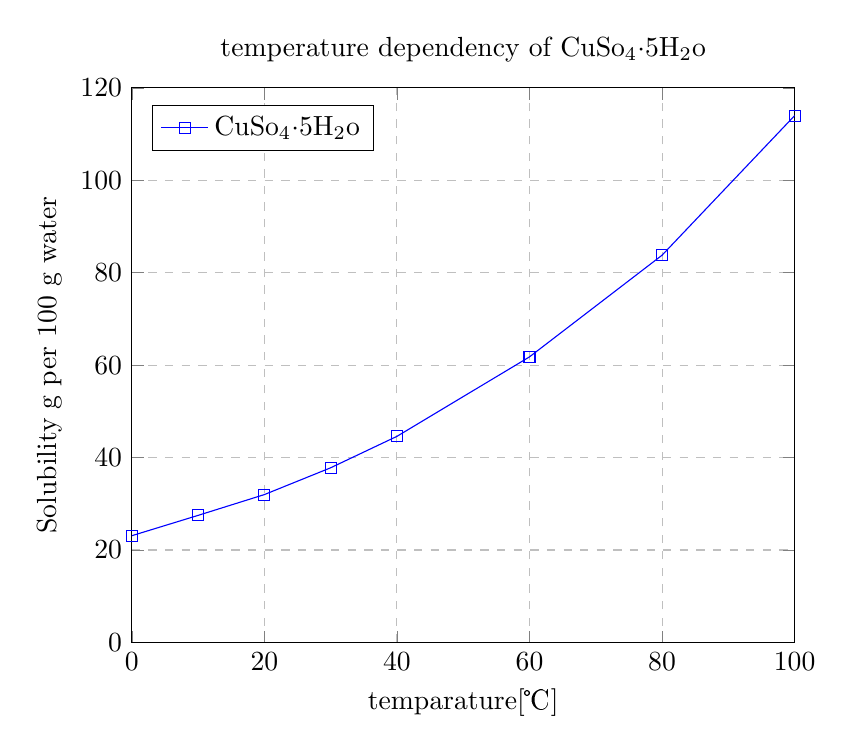
\begin{tikzpicture}
 \begin{axis}[title={temperature dependency of CuSo\(_4\cdot\)5H\(_2\)o},xlabel={temparature[\textcelsius]},
 ylabel={Solubility g  per 100 g water},
 xmin=0,xmax=100,ymin=0,ymax=120,xtick={0,20,40,60,80,100},
 ytick={0,20,40,60,80,100,120},legend pos=north west,xmajorgrids=true,ymajorgrids=true, grid style=dashed,]
 \addplot[color=blue,mark=square]coordinates{(0,23.1)(10,27.5)(20,32)(30,37.8)(40,44.6)(60,61.8)(80,83.8)(100,114)};
 \addlegendentry{CuSo\(_4\cdot\)5H\(_2\)o};
 \end{axis}
\end{tikzpicture}

%scatter plot(when computing statistical regression)
\begin{tikzpicture}
   \begin{axis}[enlargelimits=false,]
  
    \addplot[only marks,scatter,mark=*,mark size=5pt]table[meta=ma]{C:/Users/Acer/TextmakerCode/Scatter_Plot_Info.dat};
    \end{axis}
  \end{tikzpicture}  
%bar grapgh
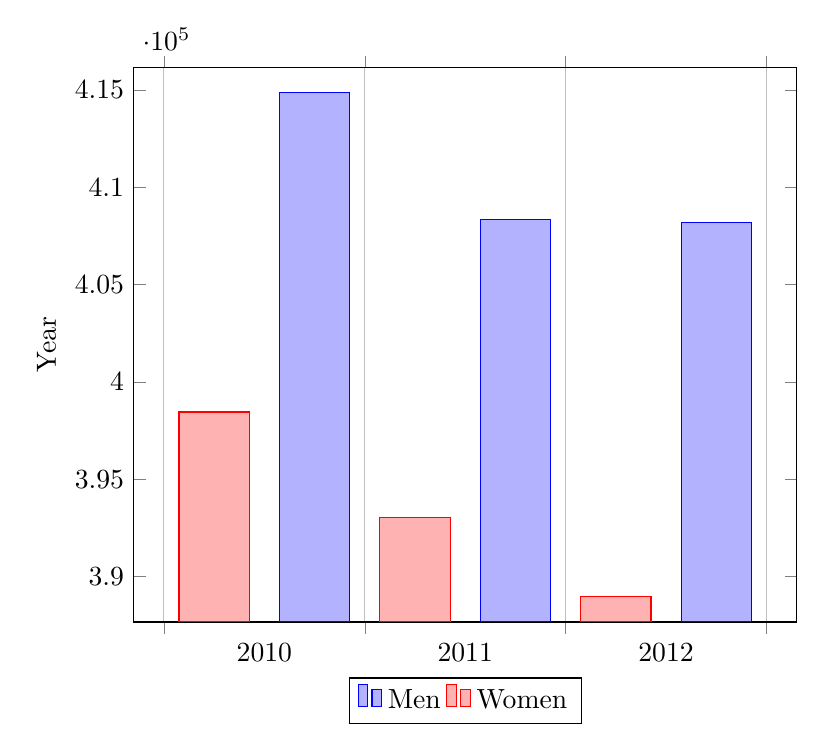
\begin{tikzpicture}
\begin{axis}[
	x tick label style={
		/pgf/number format/1000 sep=},
	ylabel=Year,
	enlargelimits=0.05,
	legend style={at={(0.5,-0.1)},
	anchor=north,legend columns=-1},
	ybar interval=0.7,
]
\addplot 
	coordinates {(2012,408184) (2011,408348)
		 (2010,414870) (2009,412156)};
\addplot 
	coordinates {(2012,388950) (2011,393007) 
		(2010,398449) (2009,395972)};
\legend{Men,Women}
\end{axis}
\end{tikzpicture}
\end{document}